\documentclass[11pt,a4paper]{article}
\usepackage[a4paper, hmargin={2.5cm,2.5cm},vmargin={2.5cm,2.5cm}]{geometry}
\usepackage{graphicx}
\usepackage{cmap}
\usepackage[utf8]{inputenc}
\usepackage[english]{babel}
\usepackage{amsmath}
\usepackage{amsfonts}
\usepackage{listings}
\usepackage{color}
\usepackage{pdfpages}
\usepackage{fancyvrb}
\usepackage{fancyhdr}
\usepackage{lipsum}
% \usepackage{pgfplots}
\usepackage{wrapfig}
\usepackage{subfig}
\usepackage{enumitem}
\usepackage{tikz}
\usepackage{forest}


\usetikzlibrary{automata, positioning, arrows}
\usetikzlibrary{positioning}
\usetikzlibrary{shapes,shapes.geometric,arrows,fit,calc}

\def\dunderline#1{\underline{\underline{#1}}}
\def\indent{\space\space\space\space}

\begin{document}
\begin{titlepage}
  \title{Programmer som data trial exam}
  \author{Albert Ross Johannessen}
  \maketitle
  \newpage
  \thispagestyle{empty}
  \newpage
\end{titlepage}

\pagestyle{fancy}
\fancyhf{}
\rhead{Programmer som data}
\rfoot{Page \thepage}
\newpage
\section{}
Betragt dette regulære udtryk over alfabetet $\{d, ','\}$, hvor $d$ står for decimalt ciffer og ',' er komma:
\begin{align}
    d+','?d*
\end{align}
Ved antagelse af, at $d$ svarer til tallene fra 0 til 9 og ',' er et komma, så beskriver det regulære udtryk kommatal.
\subsection{}
Udtrykket kan beskrive tal i sættet $\mathbb{R}^+_0$, dette vil altså sige vilkårligt store reelle tal.\\
Følgende eksempler er inkluderet i sættet:
\begin{itemize}
    \item $0$
    \item $1,1$
    \item $9,999999999$
    \item $20$
    \item $123456,0$
    \item $2,$
\end{itemize}
\subsection{}
\begin{figure}[!ht]\label{fig:examfig}
    \centering
    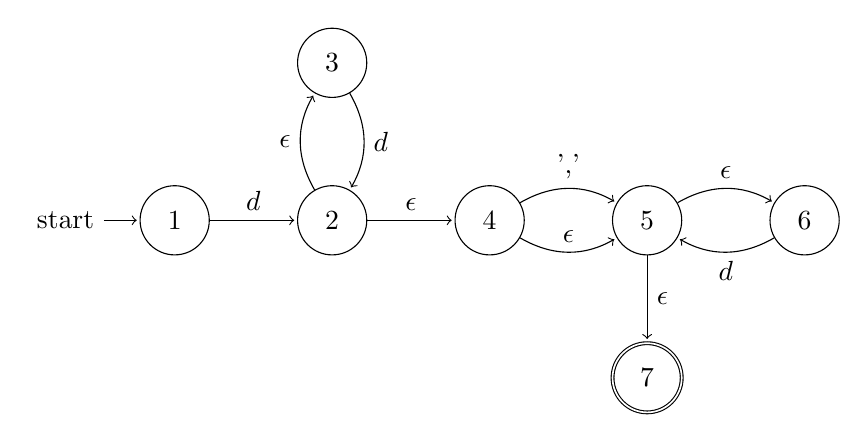
\begin{tikzpicture}[shorten >=1pt,node distance=2cm,on grid,auto] 
       \node[state, initial] (q_0)   {$1$}; 
        \node[state] (q_1) [ right =of q_0] {$2$};
        \node[state] (q_2) [above =of q_1] {$3$};
        \node[state] (q_3) [right =of q_1] {$4$};
        \node[state] (q_4) [right =of q_3] {$5$};
        \node[state] (q_5) [right =of q_4] {$6$};
        \node[state, accepting] (q_6) [below =of q_4] {$7$};
              
        \path[->] 
        (q_0) edge  node {$d$} (q_1)
        (q_1) edge [bend left] node {$\epsilon$} (q_2)
        (q_2) edge [bend left] node {$d$} (q_1)
        (q_1) edge node {$\epsilon$} (q_3)
        (q_3) edge [bend left] node {','} (q_4)
        (q_3) edge [bend right] node {$\epsilon$} (q_4)
        (q_4) edge node {$\epsilon$} (q_6)
        (q_4) edge [bend left] node {$\epsilon$} (q_5)
        (q_5) edge [bend left] node {$d$} (q_4)
        ;
    \end{tikzpicture}
    \caption{The labeled NFA representing $d+$}
\end{figure}
\subsubsection{Vil tilstandsmaskinen acceptere netop de strenge, som genkendes af det regulære udtryk ovenfor?}
Ja man kan dele det regulære udtryk op i diskrete dele. Dette kan vi sammenligne med tilstandsmaskinen angivet nedenfor.\\
\begin{figure}[!ht]\label{fig:dplus}
    \centering
    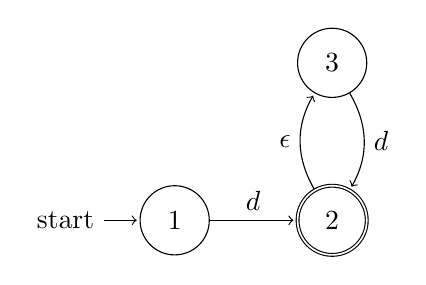
\begin{tikzpicture}[shorten >=1pt,node distance=2cm,on grid,auto] 
       \node[state, initial] (q_0)   {$1$}; 
        \node[state, accepting] (q_1) [ right =of q_0] {$2$};
        \node[state] (q_2) [above =of q_1] {$3$};
              
        \path[->] 
        (q_0) edge  node {$d$} (q_1)
        (q_1) edge [bend left] node {$\epsilon$} (q_2)
        (q_2) edge [bend left] node {$d$} (q_1)
        ;
    \end{tikzpicture}
    \caption{The labeled NFA representing $d+$}
\end{figure}
\begin{figure}[!ht]\label{fig:comma}
    \centering
    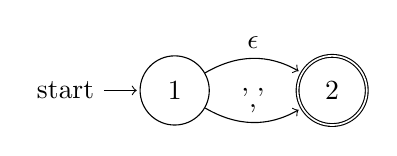
\begin{tikzpicture}[shorten >=1pt,node distance=2cm,on grid,auto] 
       \node[state, initial] (q_0)   {$1$}; 
        \node[state, accepting] (q_1) [ right =of q_0] {$2$};
              
        \path[->] 
        (q_0) edge [bend right] node {','} (q_1)
        (q_0) edge [bend left] node {$\epsilon$} (q_1)
        ;
    \end{tikzpicture}
    \caption{The labeled NFA representing $','?$}
\end{figure}
\begin{figure}[!ht]\label{fig:dopt}
    \centering
    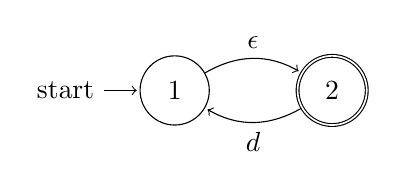
\begin{tikzpicture}[shorten >=1pt,node distance=2cm,on grid,auto] 
       \node[state, initial] (q_0)   {$1$}; 
        \node[state, accepting] (q_1) [ right =of q_0] {$2$};
              
        \path[->] 
        (q_1) edge [bend left] node {$d$} (q_0)
        (q_0) edge [bend left] node {$\epsilon$} (q_1)
        ;
    \end{tikzpicture}
    \caption{The labeled NFA representing $d*$}
\end{figure}
Det er åbenlyst at se at disse alle er dele af den tilstandsmaskine angivet.\\\\
Tilstandsmaskinen angivet er ikke deterministisk da man kan være i flere knuder på en gang på grund af eksistensen af epsilon kanter.
\newpage
\subsection{}
\begin{align}
    (d+','?d*)?
\end{align}
\subsection{}
Løsningen kan findes i kommatal.fsl
\section{}
\begin{verbatim}
let exam2_1 = Every(Write(FromTo(1, 6)));

let exam2_2 = Every(
  Write(
    Prim("+", 
      Prim("*", CstI 10, FromTo(3, 6)),
      FromTo(3,4)
    )
  )
)

let exam2_3 = Every(Write(FromToBy(1, 10, 3)))

let exam2_4 = Every(
  Write(
    Prim("+", 
      FromToBy(30, 60, 10),
      FromTo(3,4)
    )
  )
)

let exam2_5 = Every(
  Write(
      FromToBy(10, 11, 0)
  )
)
\end{verbatim}
\section{}
\begin{verbatim}
type expr = 
    | CstI of int
    | CstB of bool
    | Var of string
    | Let of string * expr * expr
    | Prim of string * expr * expr
    | If of expr * expr * expr
    | Letfun of string * string * expr * expr    (* (f, x, fBody, letBody) *)
    | Call of expr * expr
    | Print of expr

let keyword s =
    match s with
    | "else"  -> ELSE 
    | "end"   -> END
    | "false" -> CSTBOOL false
    | "if"    -> IF
    | "in"    -> IN
    | "let"   -> LET
    | "not"   -> NOT
    | "then"  -> THEN
    | "true"  -> CSTBOOL true
    | "print" -> PRINT
    | _       -> NAME s

%token ELSE END FALSE IF IN LET NOT THEN TRUE PRINT

Expr:
    AtExpr                              { $1                     }
  | AppExpr                             { $1                     }
  | IF Expr THEN Expr ELSE Expr         { If($2, $4, $6)         }
  | MINUS Expr                          { Prim("-", CstI 0, $2)  }
  | Expr PLUS  Expr                     { Prim("+",  $1, $3)     }
  | Expr MINUS Expr                     { Prim("-",  $1, $3)     }
  | Expr TIMES Expr                     { Prim("*",  $1, $3)     }
  | Expr DIV   Expr                     { Prim("/",  $1, $3)     } 
  | Expr MOD   Expr                     { Prim("%",  $1, $3)     }
  | Expr EQ    Expr                     { Prim("=",  $1, $3)     }
  | Expr NE    Expr                     { Prim("<>", $1, $3)     }
  | Expr GT    Expr                     { Prim(">",  $1, $3)     }
  | Expr LT    Expr                     { Prim("<",  $1, $3)     }
  | Expr GE    Expr                     { Prim(">=", $1, $3)     }
  | Expr LE    Expr                     { Prim("<=", $1, $3)     }
  | PRINT      Expr                     { Print($2)              }
;

| Print(ex) -> 
let evaluated = eval ex env
printfn "%A" evaluated
evaluated;;
\end{verbatim}
\section{}

\end{document}